% The first argument is the \documentclass, which tells latex which template
% we're using to build this document. It's usually safe to just use "article".
\documentclass{article}

% include some packages...
\usepackage{fullpage} % change settings for a smaller margin
\usepackage{graphicx} % gives access to the \includegraphics commands
\usepackage{amsfonts}
\usepackage{float}
\usepackage{enumitem}
\usepackage{caption}
\usepackage[export]{adjustbox}
\usepackage{bookmark}
\graphicspath{{./images/}}

% tell Latex to use no paragraph indentation, but leave some space between
% paragraphs
\setlength{\parindent}{0in}
\setlength{\parskip}{0.1in}

\newcommand{\tib}[1]{\textit{\textbf{#1}}}
\newcommand{\code}[1]{\texttt{#1}}

% these commands merely set the values for the title/date/author; they don't put
% them in the document... see \maketitle below
\title{CS Department Automated Information Timeline \\ Assignment 7.2: OCL}
\date{\today}
\author{Matthew Hays, Pawan Bhandari, Sarah Faron, Tim Klimpel \\ The Incredibles}

% all document content goes between \begin{document} and \end{document}
\begin{document}

% this command actually creates the title/date/author in the document
\maketitle
\newpage
\tableofcontents
\listoffigures
\newpage
\section{Introduction}
\subsection{Purpose}
The purpose of this assignment is to collaborate as a team to identify the three most challenging constraints in the design of the CS Department Automated Information Timeline project and describe them using OCL. The team (aka The Incredibles) met multiple times over the course of a few days to work together and identify the constraints in the design.

\section{Identifying Constraints}
\begin{enumerate}
    \item The Office Manager can only stage approved posts.
    \item The main display cannot display more than 10 posts, and all displayed posts must be approved.
    \item A notification can only be associated with one post, media, or event.
\end{enumerate}

\section{Describing Constraints with OCL}

\subsection{Constraint 1: Staging Approved Posts}

The Office Manager can only stage approved posts. \\

\{\textbf{context:} Post::tagPost():Post \\
\textbf{inv:} self.approvalStatus = ItemStatus.APPROVED\} \\

\subsection{Constraint 2: Displaying Posts}

The main display cannot display more than 10 posts, and all displayed posts must be approved. \\

\{\textbf{context:} PostController::displayPosts(): Set$<$Post$>$ \\
\textbf{inv:} let posts = self.getApprovedPosts(): Set$<$Posts$>$ \\
\textbf{inv:} posts$\rightarrow$size() $\leq$ 10 \\
\textbf{inv:} posts$\rightarrow$forEach(p | p.approvalStatus = ItemStatus.APPROVED)\} \\

\subsection{Constraint 3: Notifications}

A notification can only be associated with one post, media, or event. \\

\{\textbf{context:} Notification \\
\textbf{inv:} (self.post $<$$>$ null xor self.media $<$$>$ null) xor (self.event $<$$>$ null)\}  \\

\section{Reference: Class Diagram}

To serve as a reference for the constraints listed and OCL written to describe them, below is the JPA Data Model of our system as of the Iteration 1 submission.

\begin{figure}[H]
    \centering
    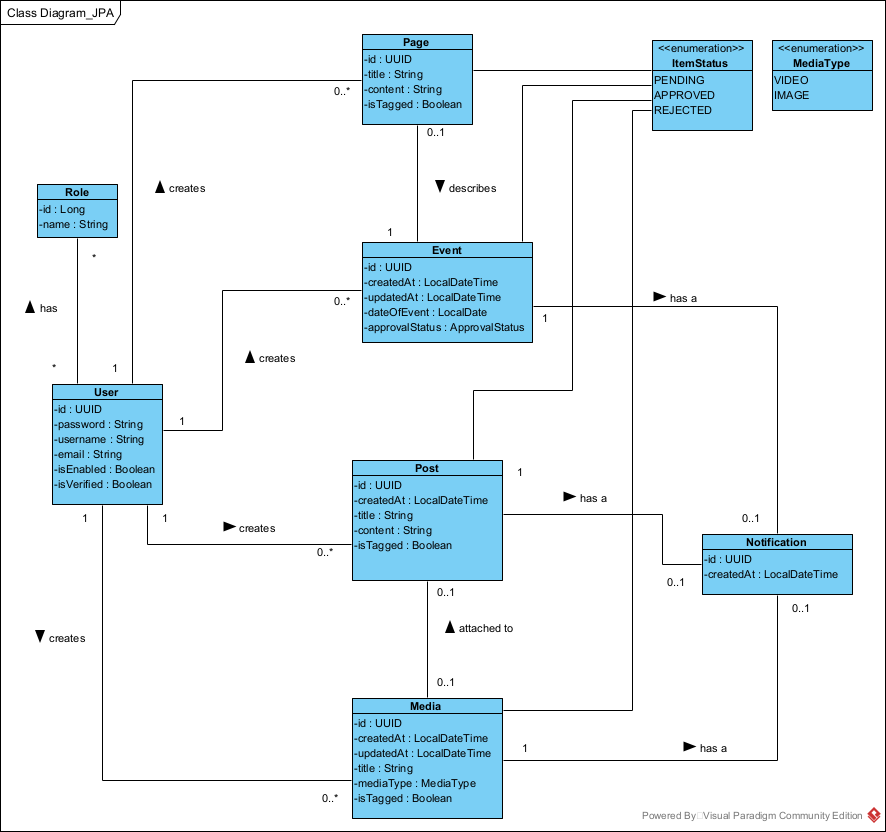
\includegraphics[width=.98\textwidth]{images/ClassDiagram.png}
    \centering
    \caption{Class Diagram}
\end{figure}

\end{document}